\section*{Problema 4}

\textbf{Este ejercicio es sobre el uso de métodos de clasificación para detectar billetes falsos:}

\begin{figure}[H]
	\centering
	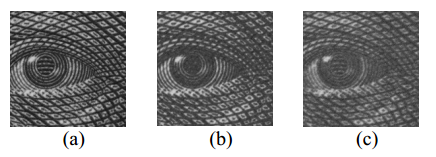
\includegraphics[width=16cm]{Graphics/Problema_04/image01.png}
	\caption{(a) (parde de) un billete de verdad, (b) billete falso de alta calidad, (c) billete falso de baja calidad.}
\end{figure}


\textbf{En el paper que se anexa a la tarea se resume cada billete con cuatro caracteristicas (varianza, skewness, curtosis y entropía) extraidas de la forma del histograma de los coeficientes de la transformación de Wavelet. Los histogramas a continuación muestran como cambia la forma cuando el billete ya no es auténtico.}

\begin{figure}[H]
	\centering
	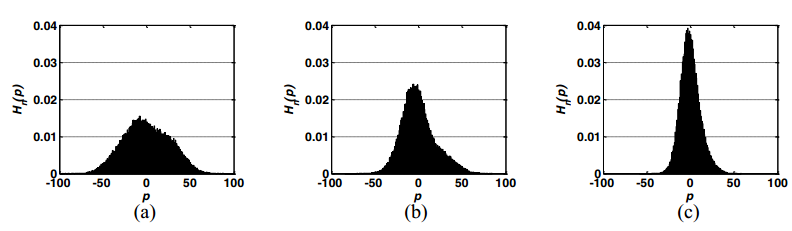
\includegraphics[width=16cm]{Graphics/Problema_04/image02.png}
	\caption{(a) histograma de los coeficientes de un billete de verdad, (b) billete falso de alta calidad, (c) billete falso de baja calidad.}
\end{figure}

\textbf{Se anexo el conjunto de datos. La última columna indica si el billete es falso o no.}

\begin{itemize}
	\item Resume, visualiza y analiza los datos
	\item Construye algunos clasificadores interesantes basados en SVM (explora diferentes kerneles). Estima su poder predictivo, para eso divide muchas veces los datos en conjunto de prueba y de entrenamiento y cuenta falsos positivos y falsos negativos. Las instrucciones básicas de SVM para R y Python están al fianl de \file{recpat4b.pdf}
\end{itemize}

\subsection*{Visualzación de datos}

En la figura \ref{fig:data_2d} se visualizan los datos de varianza, skewness y curtosis por medio de planos.

\begin{figure}[H]
    \centering
    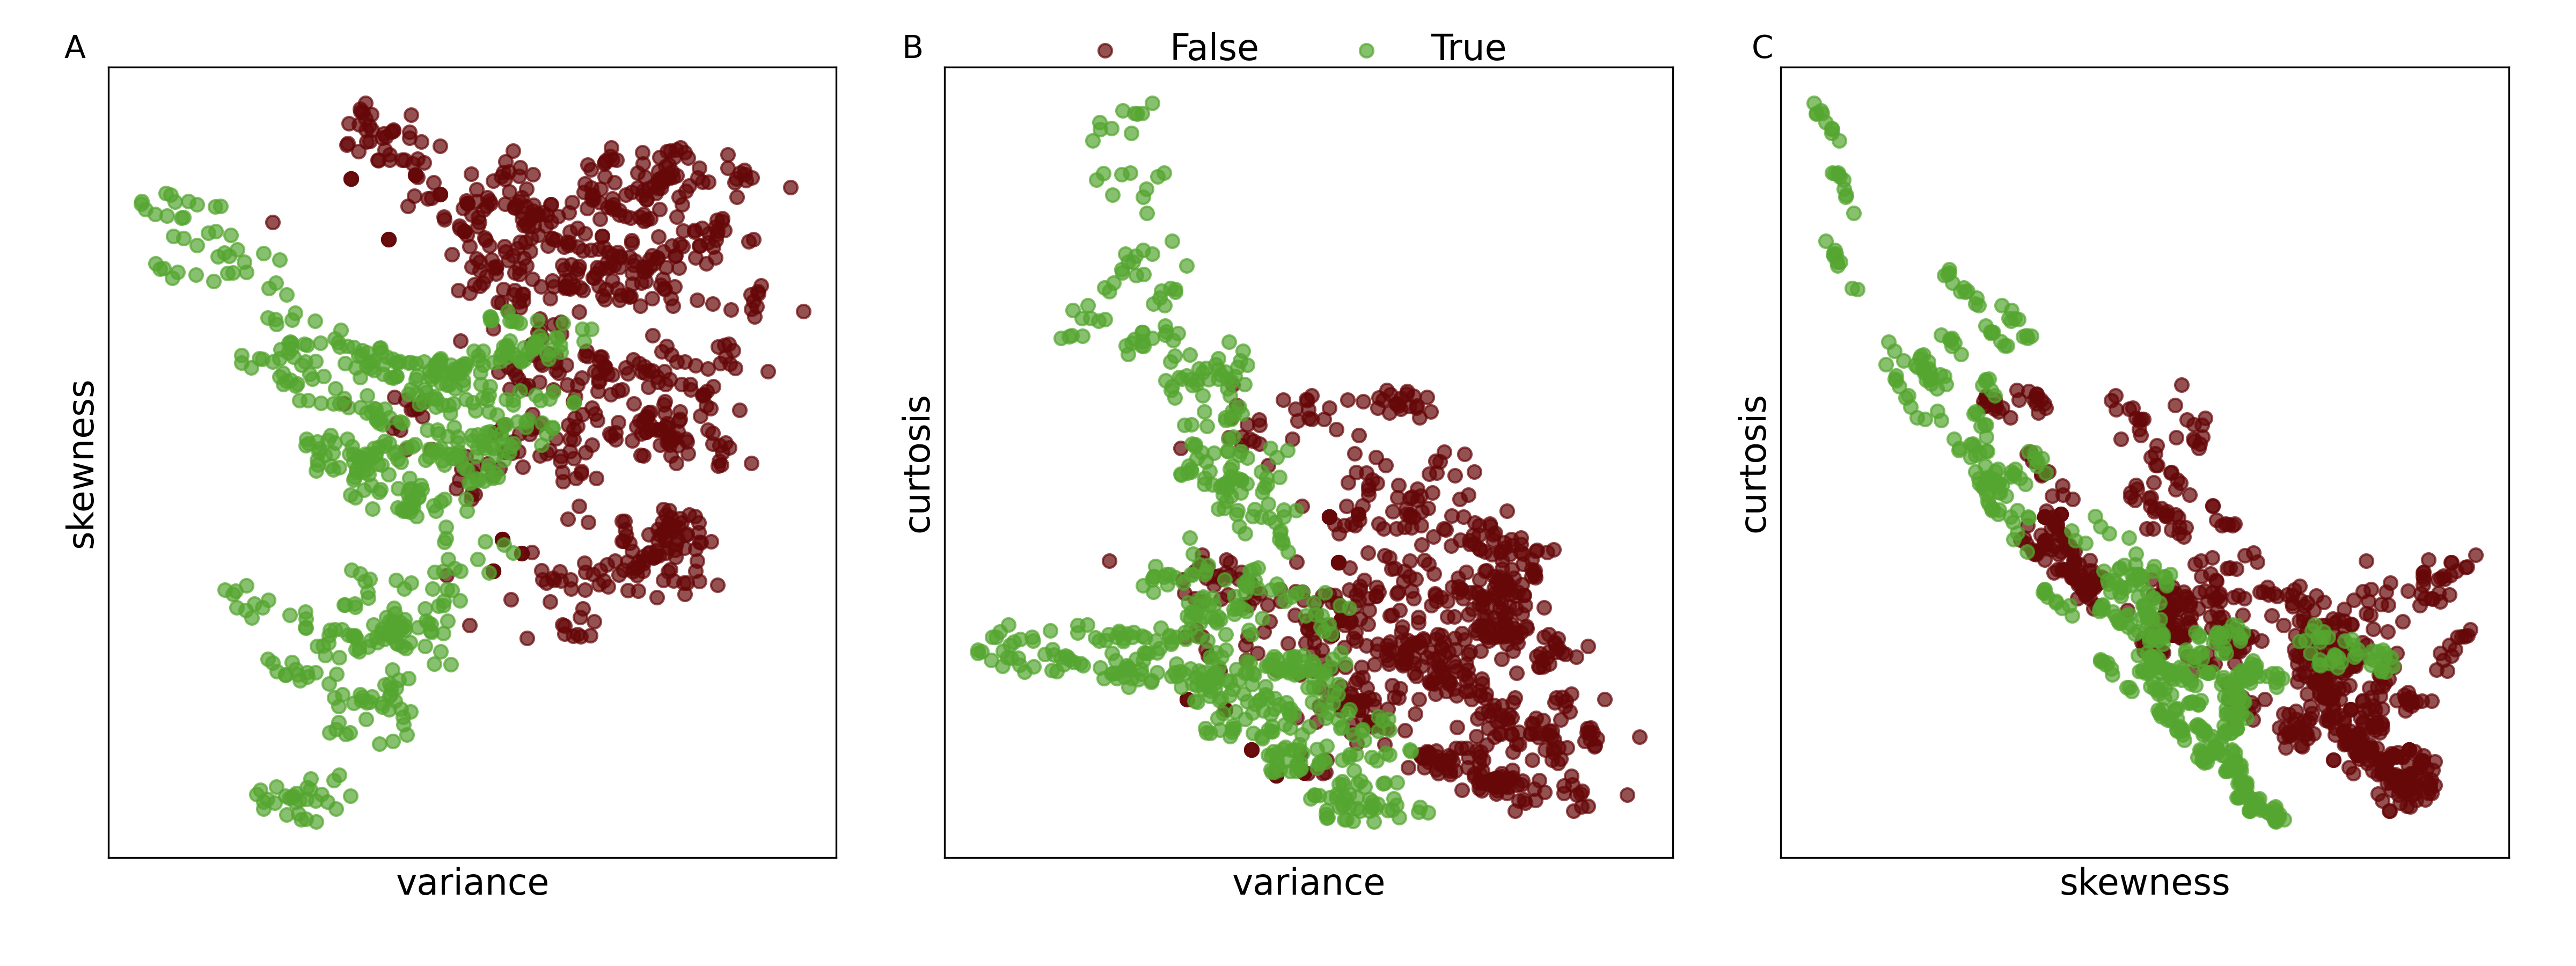
\includegraphics[width=16cm]{Graphics/Problema_04/plot_2D.png}
    \caption{Visualización por planos de los datos de varianza, skewness y curtosis.}
    \label{fig:data_2d}
\end{figure}

La configuración donde se obtiene una mayor diferencia entre cada conjunto de billetes es en el plano de la varianza y la curtosis. En la figura \ref{fig:data_3d} se visualizan los datos usando cada característica para los planos. En esta visualización se logra apreciar de mejor manera que existe una separación entre los dos tipos de billetes.

\begin{figure}[H]
    \centering
    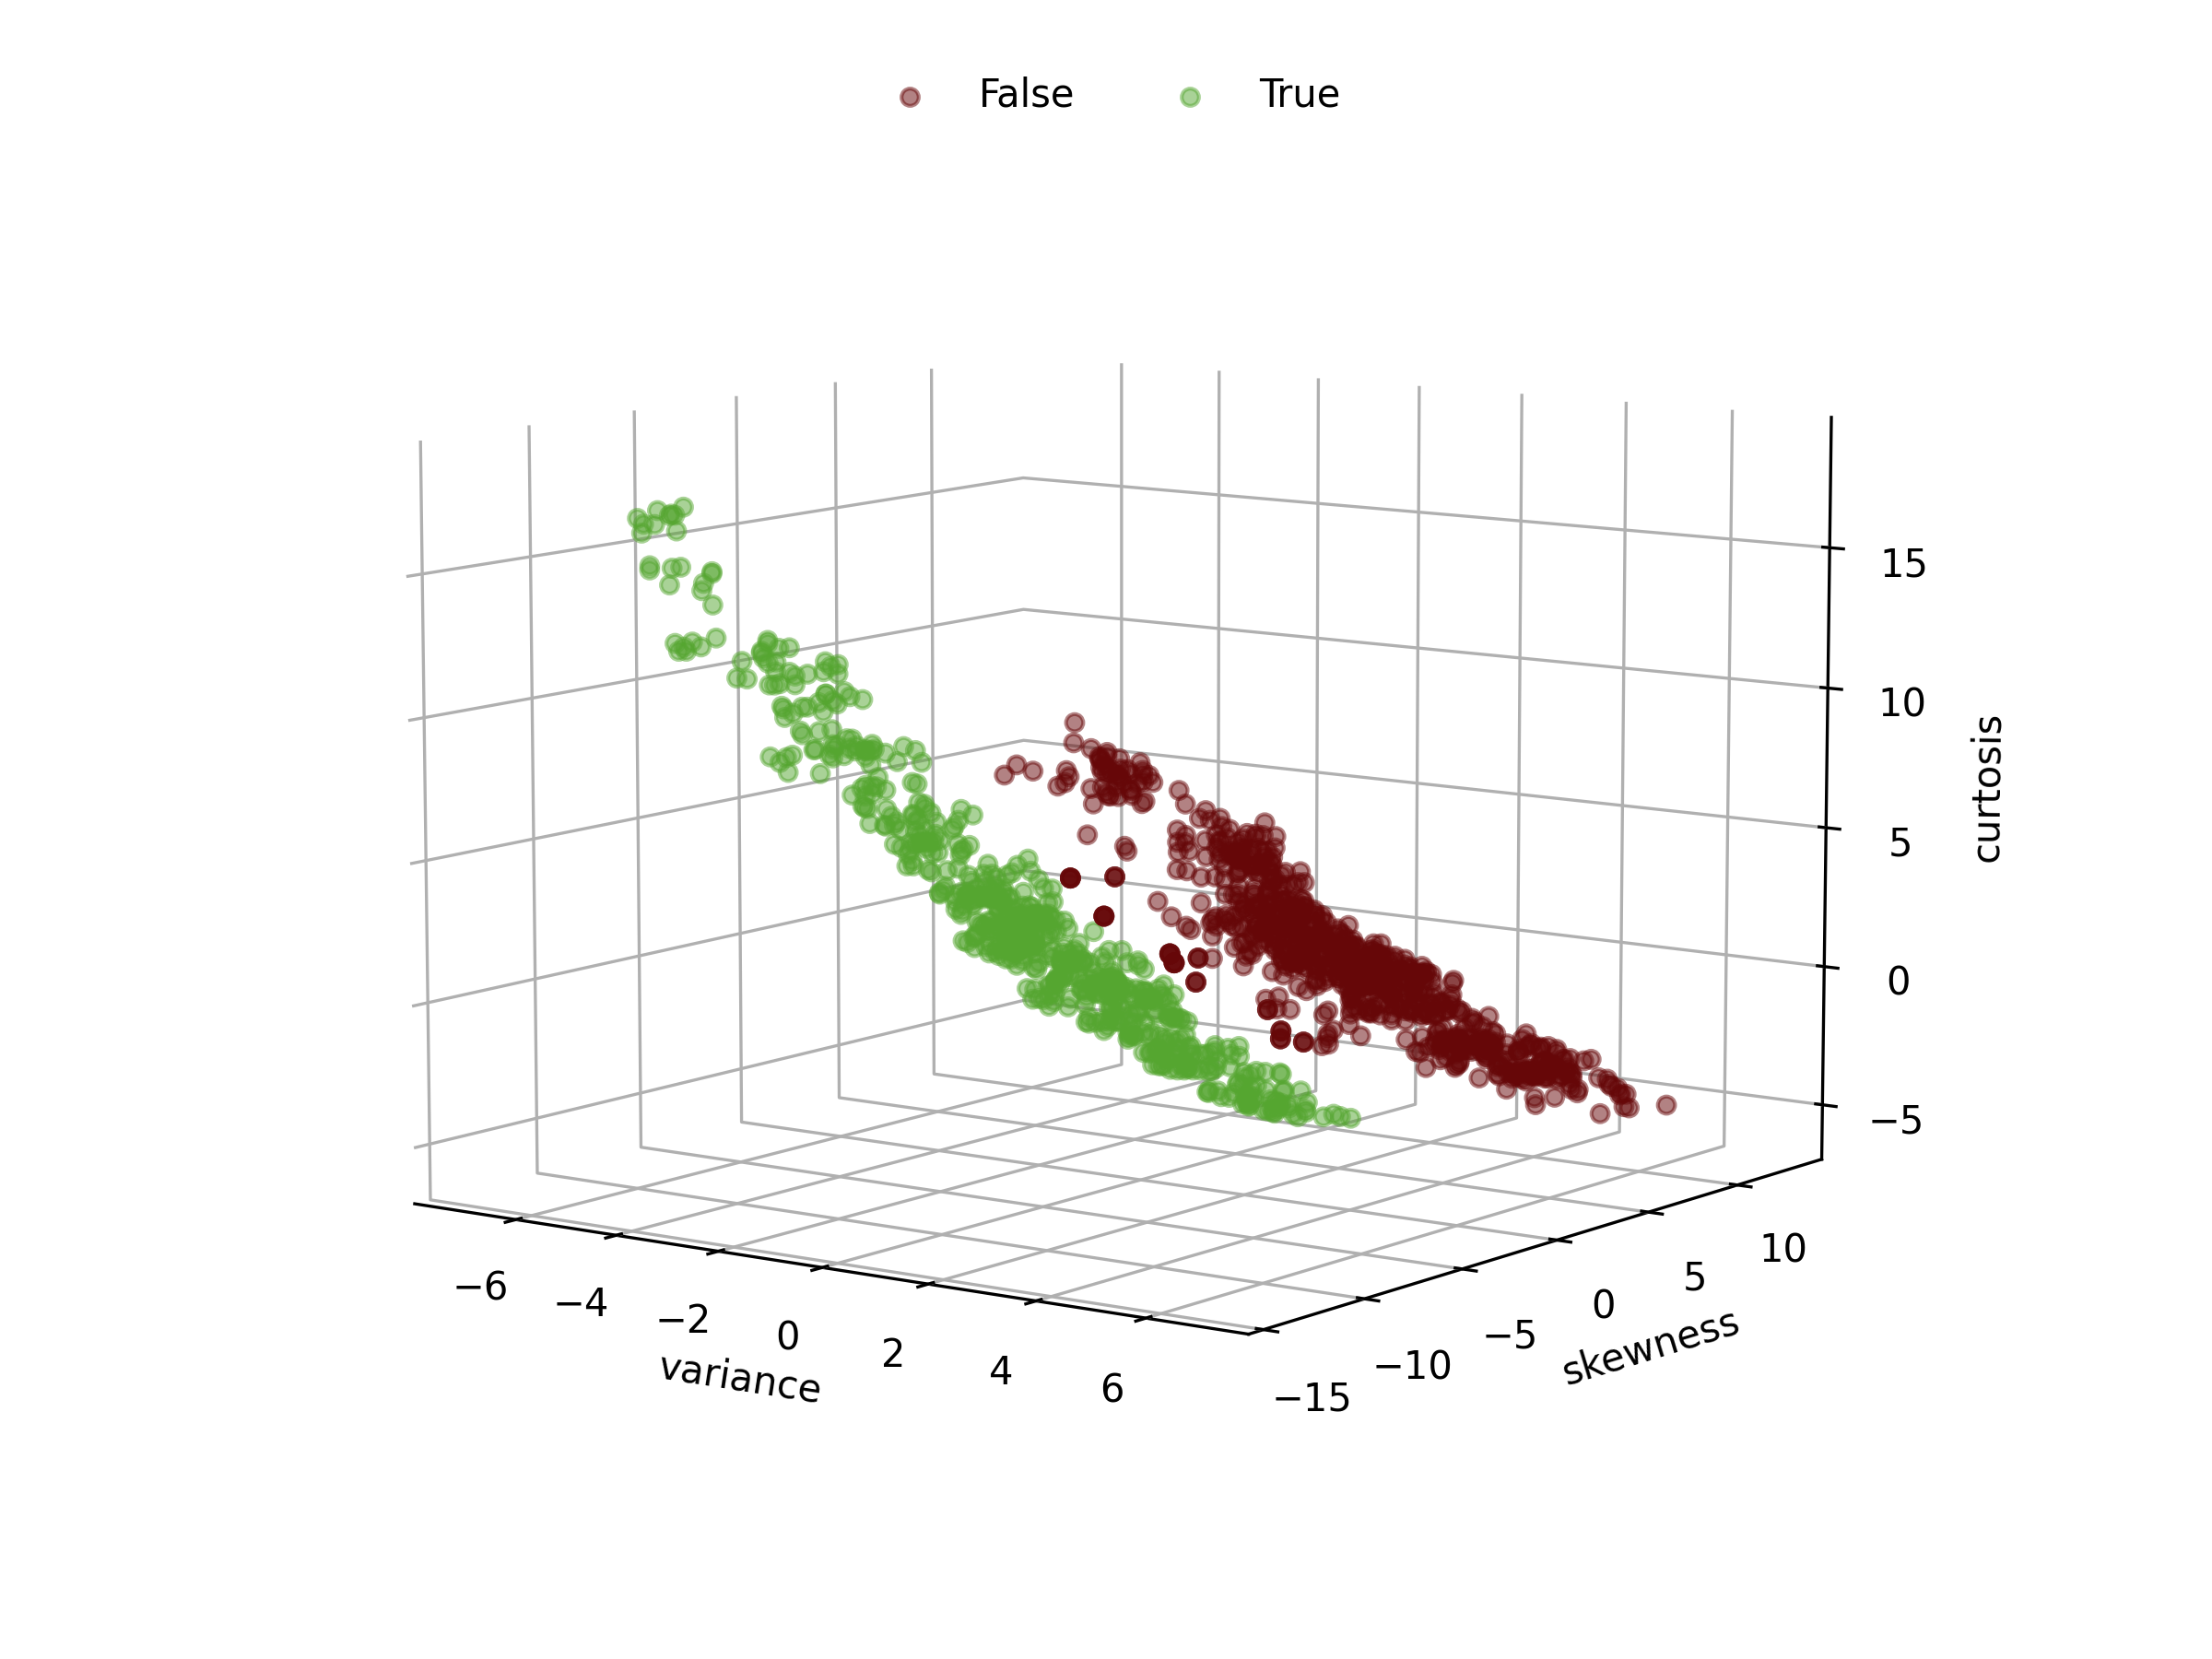
\includegraphics[width=16cm]{Graphics/Problema_04/plot_3D.png}
    \caption{Representación gráfica de los datos usando cada característica como un plano.}
    \label{fig:data_3d}
\end{figure}

Sea $X$ una matriz con las caracteristicas de cada billete donde $X\in R^{n\times 3}$ donde $n$ es el número de billetes caracterizados. Se utilizo la matriz $XX^T$ para iniciar el método de PCA con kernel lineal para obtener un conjunto de datos de dimensión $n\times 3$. En la figura \ref{fig:pca_2d} se visualizan las tres componentes principales obtenidas usando las combinaciones posibles en un plano bidimensional.

\begin{figure}[H]
    \centering
    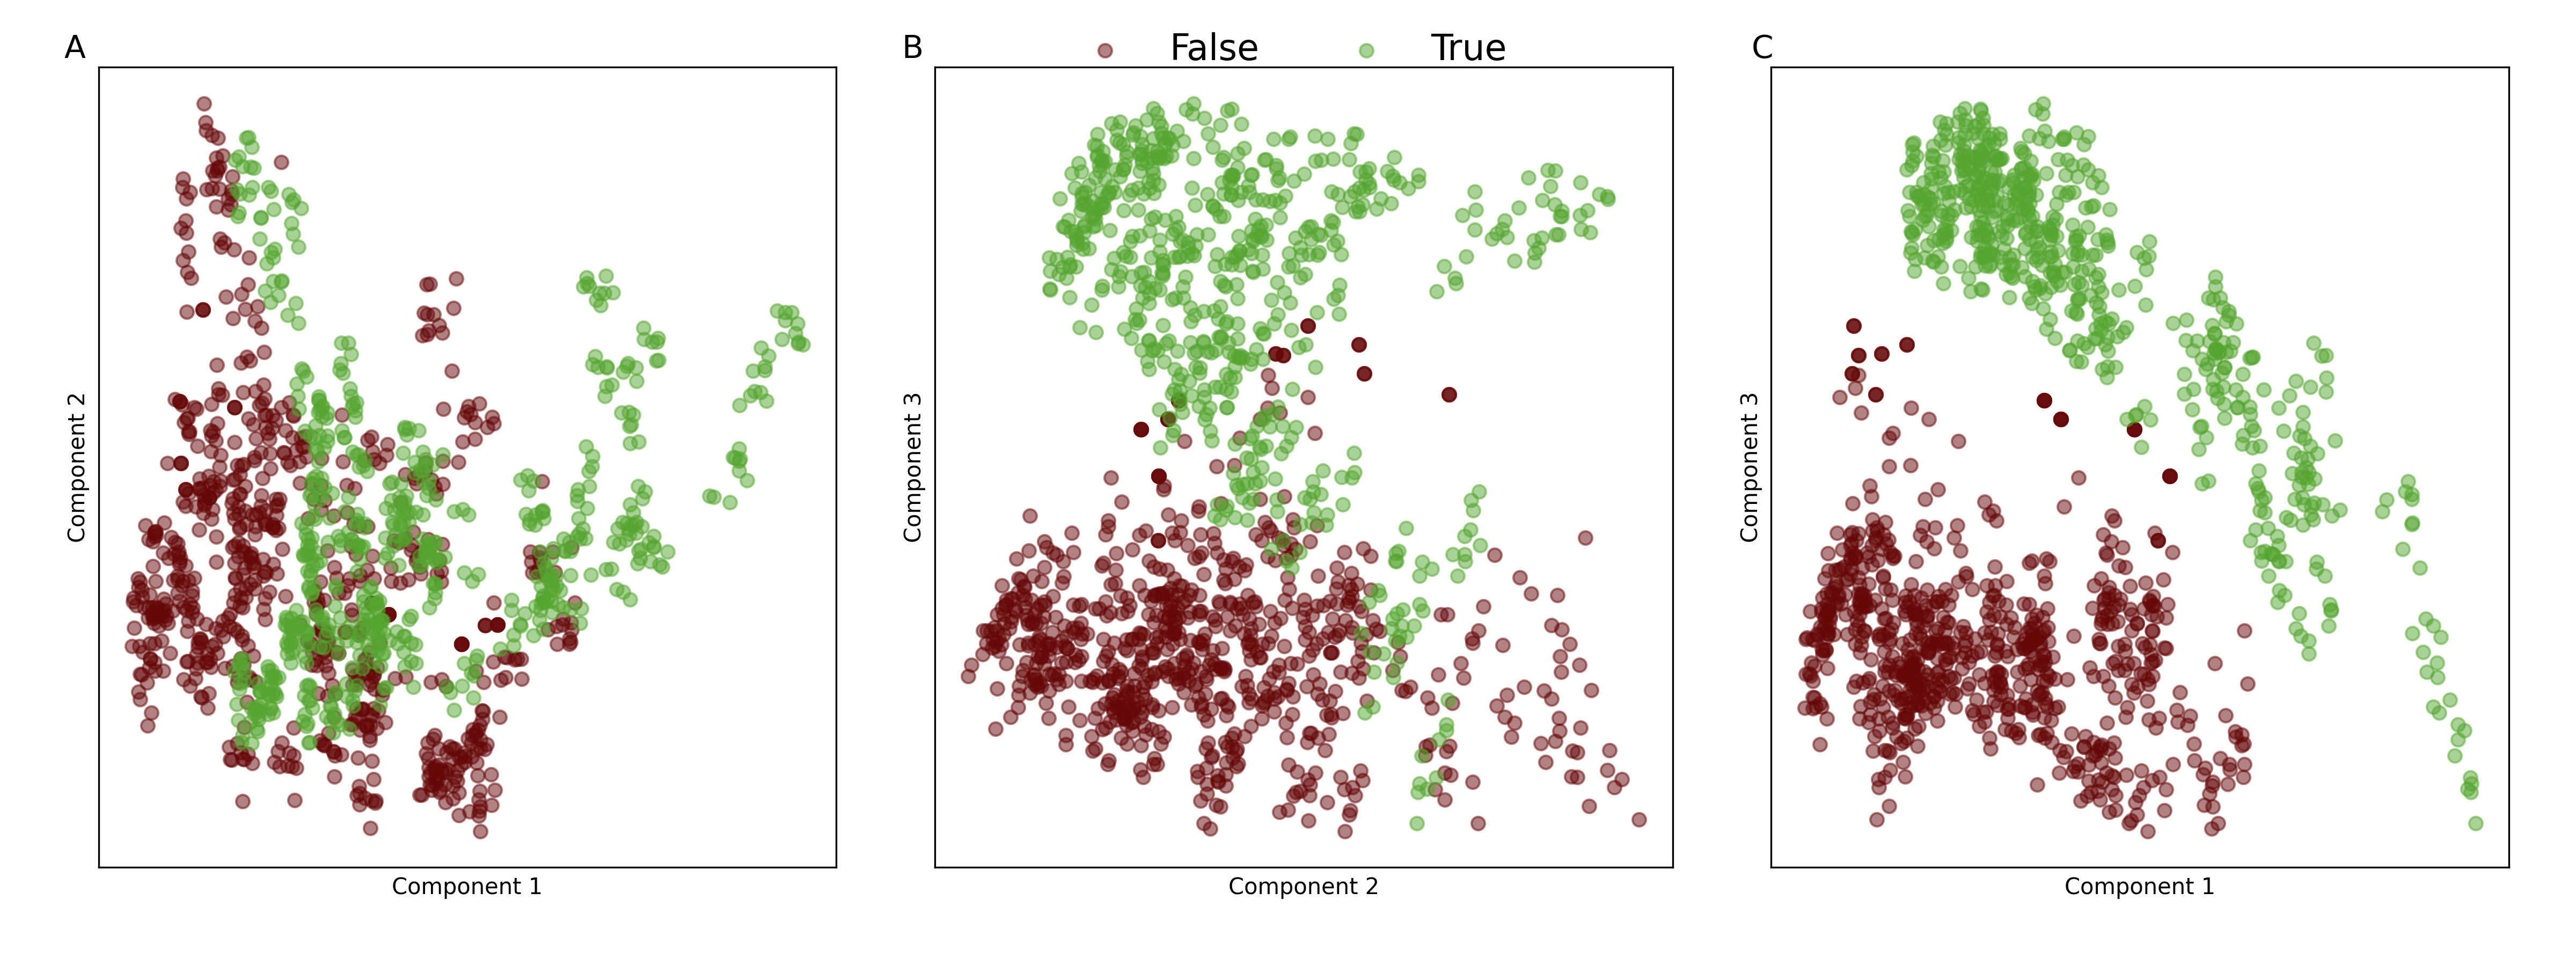
\includegraphics[width=16cm]{Graphics/Problema_04/PCA_2D.png}
    \caption{Representación gráfica de las tres componentes principales obtenidas de PCA usando la matriz $XX^T$.}
    \label{fig:pca_2d}
\end{figure}

Con esta representación se observa que existe una mayor distinción cuando la primer y tercer componentes son usadas como planos. En la figura \ref{fig:pca_3d} se visualizan las tres componentes obtenidas del método de PCA, cada componente usando un plano.

\begin{figure}[H]
    \centering
    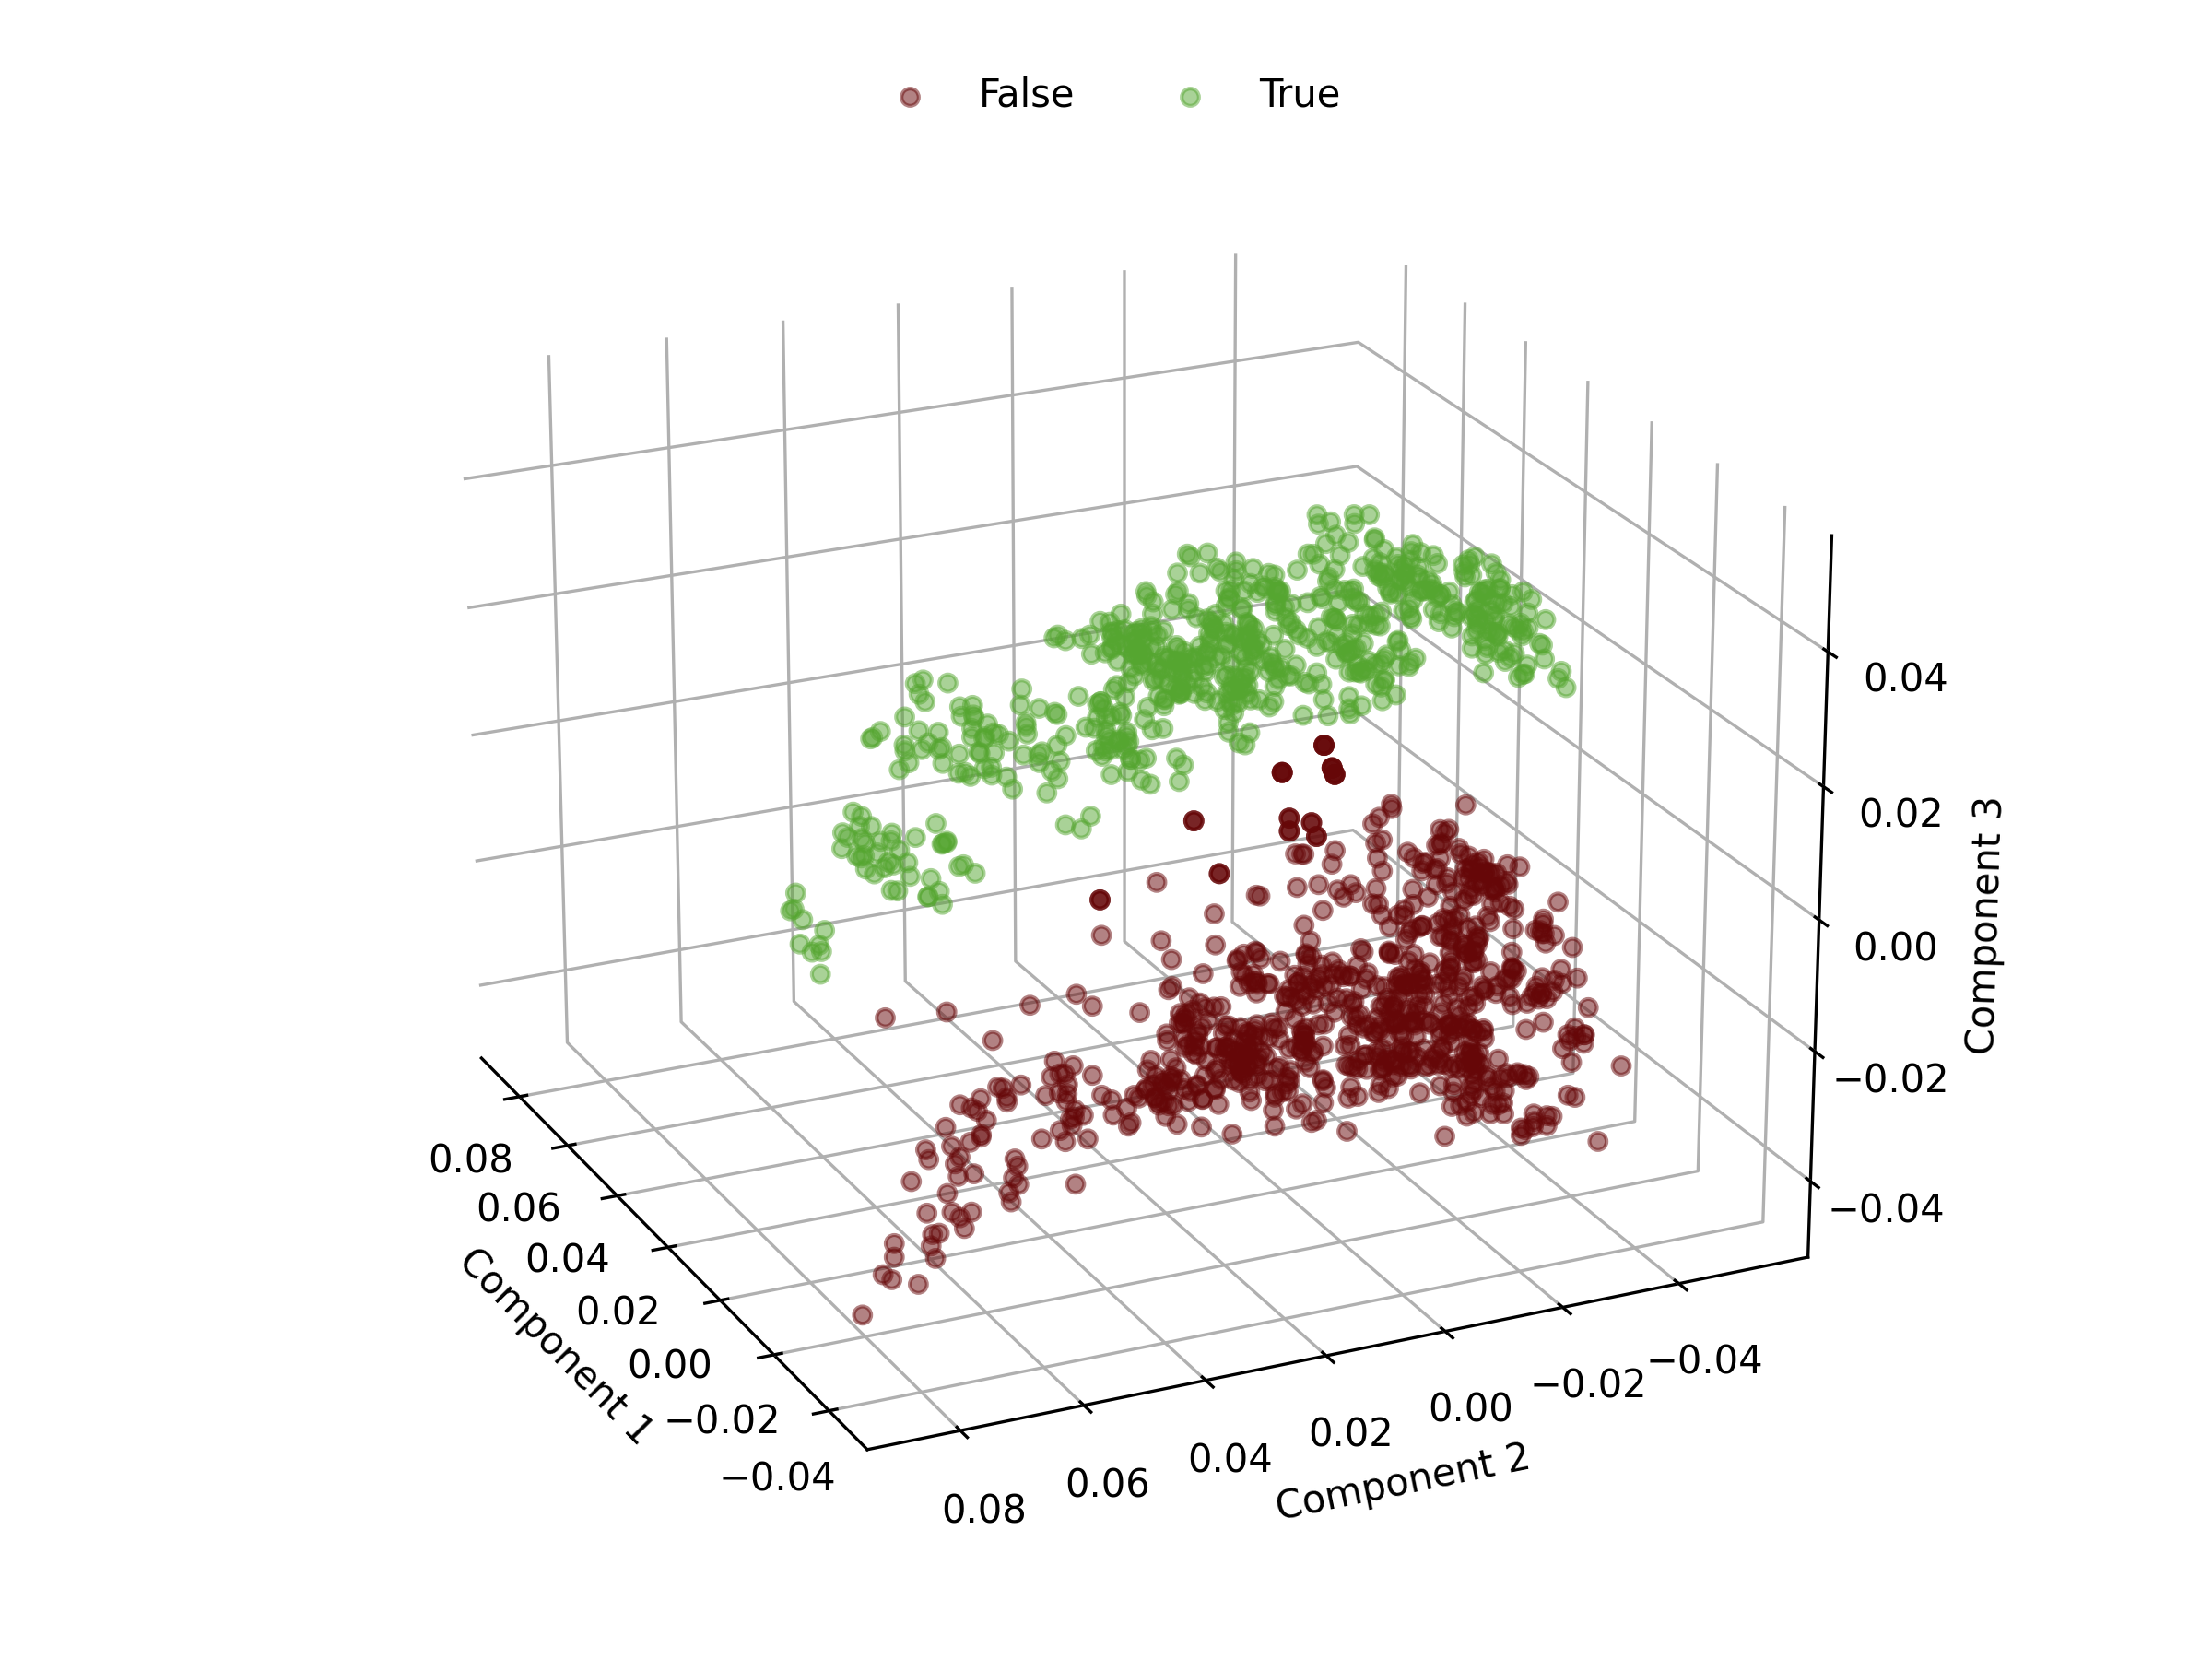
\includegraphics[width=16cm]{Graphics/Problema_04/PCA_3D.png}
    \caption{Representación gráfica de las tres componentes principales obtenidas de PCA usando cada componente como un plano.}
    \label{fig:pca_3d}
\end{figure}

Con esta representación se obtiene de igual manera una distinción entre cada conjutno de billetes. En comparación con la figura \ref{fig:data_3d}, se observa una mayor disperción en los datos.

Para el método de SVM se usaron el kernel lineal, polinomial, rbf y sigmoide. En la tabla \ref{table:parameters} se encuentean los parámetos de cada kernel usado.


\begin{table}[H]
    \centering
    \begin{tabular}{cccc} \hline
        Kernel     & Grado & $\gamma$              & $r$ \\ \hline
        Lineal     & -     & -                     & -   \\
        Polinomial & 3     & $\frac{1}{n\sigma^2}$ & 0   \\
        RBF        & -     & $\frac{1}{n\sigma^2}$ & -   \\
        Sigmoide   & -     & $\frac{1}{n\sigma^2}$ & 0   \\ \hline
    \end{tabular}
    \caption{Parámetros usados para cada kernel. El simbolo $-$ indica que no es necesario el parámetro en el kernel.}
    \label{table:parameters}
\end{table}


Se realizo una partición del conjunto de datos $X$. En esta partición de considero el 90\% como datos de entrenamiento y 10\% como datos de validación. Con los datos de validación se obtuvo un puntaje de accuracy. En la tabla \ref{table:data_2d} se encuentran los resultados de aplicar SVM y los datos $X$ como se muestran en la figura \ref{fig:data_2d}.

\begin{table}[H]
    \centering
    \begin{tabular}{lcccc} \hline
        Figura & Lineal & Polinomial & RBF   & Sigmoide \\ \hline
        A      & 0.674  & 0.645      & 0.819 & 0.558    \\
        B      & 0.927  & 0.906      & 0.899 & 0.811    \\
        C      & 0.978  & 1.000      & 1.000 & 0.877    \\ \hline
    \end{tabular}
    \caption{Puntajes de accuracy para las configuraciones mostradas en la figura \ref{fig:data_2d}.}
    \label{table:data_2d}
\end{table}

Estos resultados pueden ser visualizados en la figura \ref{fig:svm_data}.

Con los datos obtenidos con PCA se obtuvieron los puntajes de accuracy mostrados en la tabla \ref{table:pca_2d}.

\begin{table}[H]
    \centering
    \begin{tabular}{lcccc} \hline
        Figura & Lineal & Polinomial & RBF   & Sigmoide \\ \hline
        A      & 0.601  & 0.754      & 0.760 & 0.565    \\
        B      & 0.927  & 0.848      & 0.920 & 0.826    \\
        C      & 0.964  & 1.000      & 1.000 & 0.862    \\ \hline
    \end{tabular}
    \caption{Puntajes de accuracy para las configuraciones mostradas en la figura \ref{fig:pca_2d}.}
    \label{table:pca_2d}
\end{table}

Estos resultados pueden ser visualizados en la figura \ref{fig:svm_pca}.

Tratando a los conjuntos de datos mostrados en las figuras \ref{fig:data_3d} y \ref{fig:pca_3d}. Se realizo una comparación de los puntajes de accuracy, porcentajes de falsos positivos y porcentajes de falsos negativos. Los resultados que se obtuvieron son mostrados en la tabla \ref{table:results_3d}.

\begin{table}[H]
    \centering
    \begin{tabular}{l|ccc|ccc} \hline
        \multirow{2}{*}{Kernel} & \multicolumn{3}{c}{Originales} & \multicolumn{3}{|c}{PCA}                                    \\ \cline{2-7}
                                & Accuracy                       & FN                       & FP    & Accuracy & FN    & FP    \\ \hline
        Lineal                  & 0.971                          & 0.014                    & 0.014 & 0.978    & 0     & 0.022 \\
        Polinomial              & 0.978                          & 0                        & 0.022 & 1.0      & 0     & 0     \\
        RBF                     & 1.0                            & 0                        & 0     & 1.0      & 0     & 0     \\
        Sigmoide                & 0.565                          & 0.21                     & 0.225 & 0.841    & 0.101 & 0.058 \\ \hline
    \end{tabular}
    \caption{Puntajes de accuracy para las configuraciones mostradas en la figura \ref{fig:data_3d} y \ref{fig:pca_3d}.}
    \label{table:results_3d}
\end{table}


Con estos resultados se obtiene que por medio de los parámetros de varianza, skewness, curtosis y las primeras tres componentes obtenidas de PCA obtenidas de los parámetros se pueden crear clasificadores eficientes para la tarea de diferenciar billetes verdaderos y billetes falsos. El mejor kernel para la tarea es el RBF con los parámetros usados en la tala \ref{table:parameters}. Para obtener una mejor clasificación es usar todos los datos para generar el kernel. Usar PCA como entrada para el modelo de SVM produce mejores resultados, sin embargo para datos de mayor longitud esto puede ser perjudicial por el tiempo de computo.

\pagebreak

\begin{figure}[H]
    \centering
    % \includegraphics[width=1\linewidth]{Graphics/Problema_04/SVM_data.png}
    \caption{Representación grafica de la clasificación de los datos de varianza, skewness y curtosis como un plano de visualización bidimensional.}
    \label{fig:svm_data}
\end{figure}

\pagebreak

\begin{figure}[H]
    \centering
    % 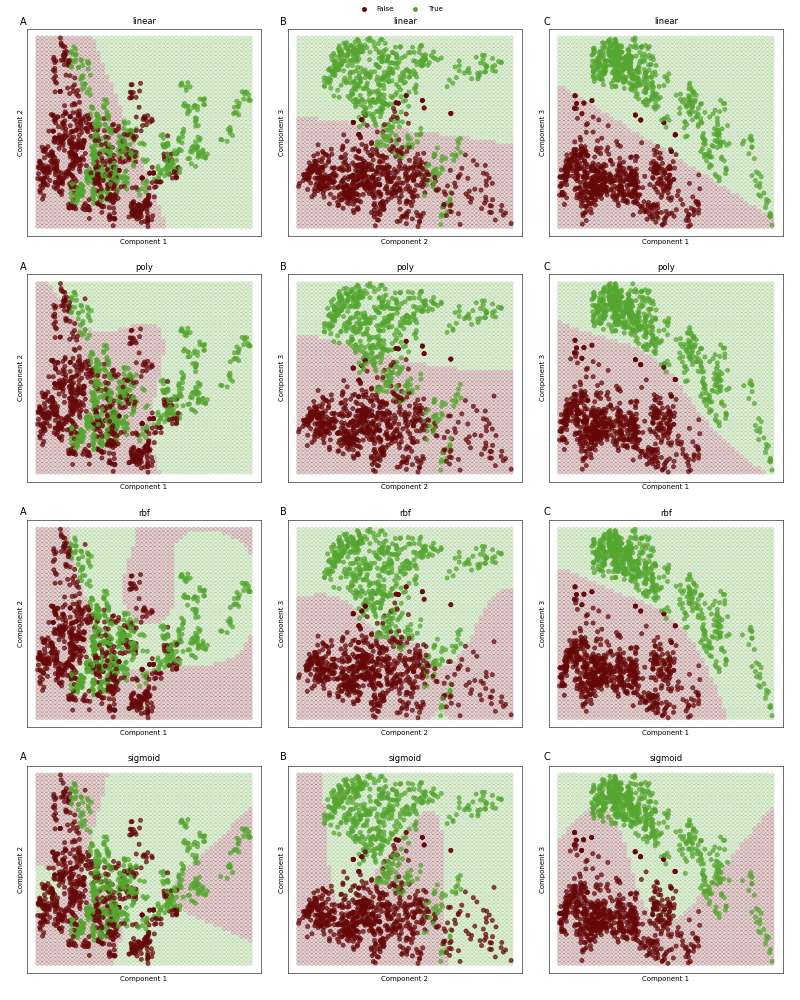
\includegraphics[width=1\linewidth]{Graphics/Problema_04/SVM_PCA.png}
    \caption{Representación grafica de la clasificación de los datos de las primeras tres componentes principales de PCA como un plano de visualización bidimensional.}
    \label{fig:svm_pca}
\end{figure}